The Rectified linear Unit (RelU) is a very simple activation function, none the less, still a very useful function. When ReLU i called with some input, it will go through all values of the input, turning all negative values to 0, and all positive number, simply keeps the value.

$$
ReLU(input) = max(0,input)
$$
or
$$
ReLU(input) =
\left\{ \begin{matrix}
		input& \geq& 0& =& input& \\
		\\
		input& <& 0& =& 0&
\end{matrix}
\right.
$$


\begin{figure}[!ht]
  \centering
  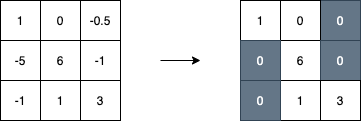
\includegraphics[scale=0.4]{latex/IMGs/relu.png}
  \caption{Shows how a 1x3 mean filter acts on a 1x9 feature map, with stride 1}\label{Baseline:before}
\end{figure}